\section{Vorlesung 11.05.2016}

\subsection{Orientierung im Raum : Die optomotorische Reaktion}

Ommatidium besteht aus 20 Zellen wobei 8 Photorezeptoren (Retinulazellen R1-R8, welche zweischichtiges Rhadomer bilden) für die Verarbeitung der visuellen Information verantwortlich sind. Adultes Komplexauge besteht aus 800 regelmäßig angeordneten, hexagonalen Einheiten (Ommatidien)\\

omb$^{H31}$-Mutation:
\begin{itemize}
	\item Optomotorische Reaktion im Flug gestört (large field response, not object response)
	\item Optomotorische Reaktion im Lauf weniger gestört
	\item Vermeidung dunkler Objekte
	\item Männliches Balzverhalten gestört
	\item Leichte Störung im Elektroretinogram (ERG)
\end{itemize}

In omb$^{H31}$-Mutation fehlen Riesenneurone der Lobulaplatte
Mutation betrifft das Gen bifid; 40kb-Deletion downstream (regulatorische Region); codiert einen Transkriptionsfaktor\\

\subsubsection{Elementarer Bewegungsdetektor}
Wahrnehmung der Luminanzgrenze erst durch Rezeptor A, dann durch Rezeptor B. Je schneller sich Grenze bewegt, je stärkeres Outputsignal (erstmals theoretisch beschrieben von Reichhardt in 1956)\\
Stimulierung des Rezeptor A, dann nach Strecke S Stimulierung des Rezeptor B. Signal A ist verzögert durch Interneuron. Komparator Neuron summiert die Signale\\
Richtung- und Geschwindigkeitsspezifisch\\
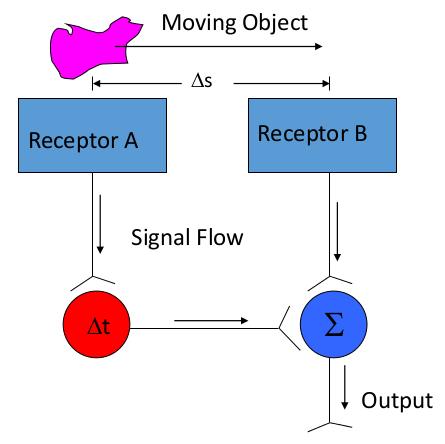
\includegraphics[width=0.6\textwidth]{lectures/160511/pix/unidirectional_motiondetection.png}

Damit beide Richtungen wahrgenommen werden können, Überkreuzschaltung\\
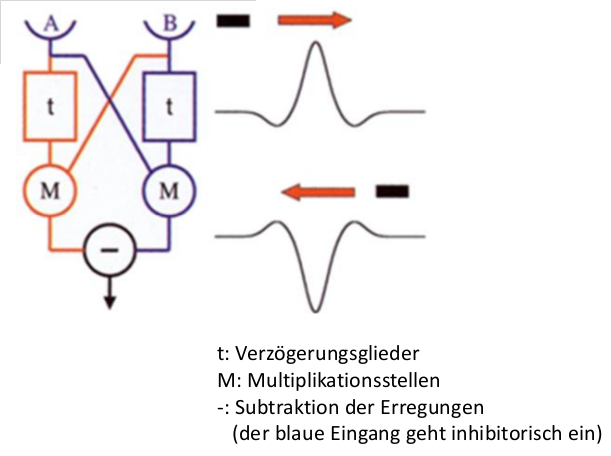
\includegraphics[width=1\textwidth]{lectures/160511/pix/bidirectional_motiondetection.png}

Mutante wird durch Kombination von Gal4-UAS-System und Shi-ts (temperaturempfindliches Protein, 30 $^\circ$C hergestellt $\rightarrow$ verhindert Endozytose synaptischer Vesikel\\
Versucht zeigt, dass L1 und L2 Zellen in Lobula Platte als Bewegungsdetekor bei Drosophila fungieren\\

\subsubsection{Augenentwicklung bei Drosophila Melanogaster}
Komplexauge besteht aus Ommatidien; jedes einzelne funktioniert als unabhängiger visueller Rezeptor. Zwei Ausrägungen:
\begin{itemize}
	\item Appositionsauge: Ommatidien funktionieren unabhängig (meiste Taginsekten)
	\item Superpositionsauge: Ommatidien kooperieren um ein helleres, überlagenderes Bild auf der Retina zu erzeugen (nachtaktive Insekten)
	\item Beim neuralen Superpositionsauge (schnellfliegende Insekten wie z. B. Drosophila) sind, wie beim Appositionsauge, die Pigmentzellen durchgängig. Im Gegensatz zum Appositionsauge und zum optischen Superpositionsauge gibt es in jedem Ommatidium kein fusioniertes Rhabdom, die zwei mittleren Rhabdomere (7 und 8) liegen hier untereinander. Die sieben einzelnen Rhabdomere sind so angeordnet, dass es ein zentrales Rhabdomer (bestehend aus den beiden Einzelrhabdomeren 7 und 8) und darum jeweils sechs periphere Rhabdomere gibt. Jedes periphere Rhabdomer ist neuronal mit dem zentralen Rhabdomer des gegenüberliegenden Ommatidiums verschaltet, weshalb dieser Augentyp als neuronales Superpositionsauge bezeichnet wird.
\end{itemize}

Ca. 800 Ommatidien mit je 20 Zellen:
\begin{itemize}
	\item 8 Rezeptorzellen
	\item 2 primäre Pigmentzellen
	\item 1 sekundäre Pigmentzelle
	\item 1 tertiäre Pigmentzelle
	\item 4 Kristallkegelzellen
	\item 4 Zellen zur Ausbildung des Haarkomplexes
\end{itemize}

Jede Zelle mit definiertem Platz, d.h. jede Zelle immer mit gleichem Kontakt zu gleichem Satz Nachbarzellen

Das Komplexauge entwickelt sich aus der Augenimaginalscheibe.\\
In der 3. Larve bewegt sich eine synchrone Mitosewelle von posterior nach anterior über die Imaginalscheibe = Start der Differenzierung.\\
Die Mitose ist mit einer Verkürzung der Zellen gekoppelt $\rightarrow$ \textbf{morphogenetische Furche}\\
Räumlicher Abstand zur Furche = Maß des Differenzierungsgrades $\rightarrow$ In einer Augenscheibe verschieden weit fortgeschrittene Stadien der Ommatidienentwicklung\\

Wie, in welcher Folge entwickeln sich verschiedene Zelltypen aus einer einschichtigen Epithel? Mitotische Rekombination:
\begin{itemize}
	\item Zellklone in der Augenscheibe, Untersuchung im Grenzbereich
	\item Zellen unterschiedlicher Herkunft werden für ein Ommatidium rekrutiert
	\item Selbst nach der letzten Teilung sind die Zellen noch nicht vollständig determiniert
	\item Induktive, d.h. auf Zell-Zell-Wechselwirkungen, beruhende Entwicklung
\end{itemize}

\subsubsection{Vorteile des Entwicklungsmodells Komplexauge}
Identische Untereinheiten in festgelegter Struktur $\rightarrow$ jeder Fehler wiederholt sich 800x\\
Mutanten mit defekten Augen / ganz ohne Augen sind unter Laborbedingungen lebensfähig\\
In Näherung zweidimensionales Muster (einschichtiges Epithel)